\documentclass{article}
\usepackage{graphicx}

\usepackage{geometry}
\geometry{hmargin=1cm,vmargin=1cm}

\usepackage{tikz}

\def\width{18}
\def\hauteur{13}

\begin{document}
	\begin{center}
		\begin{tikzpicture} [x=1cm, y=1cm, semitransparent]
		\node[anchor=south west,inner sep=0] at (0,0) {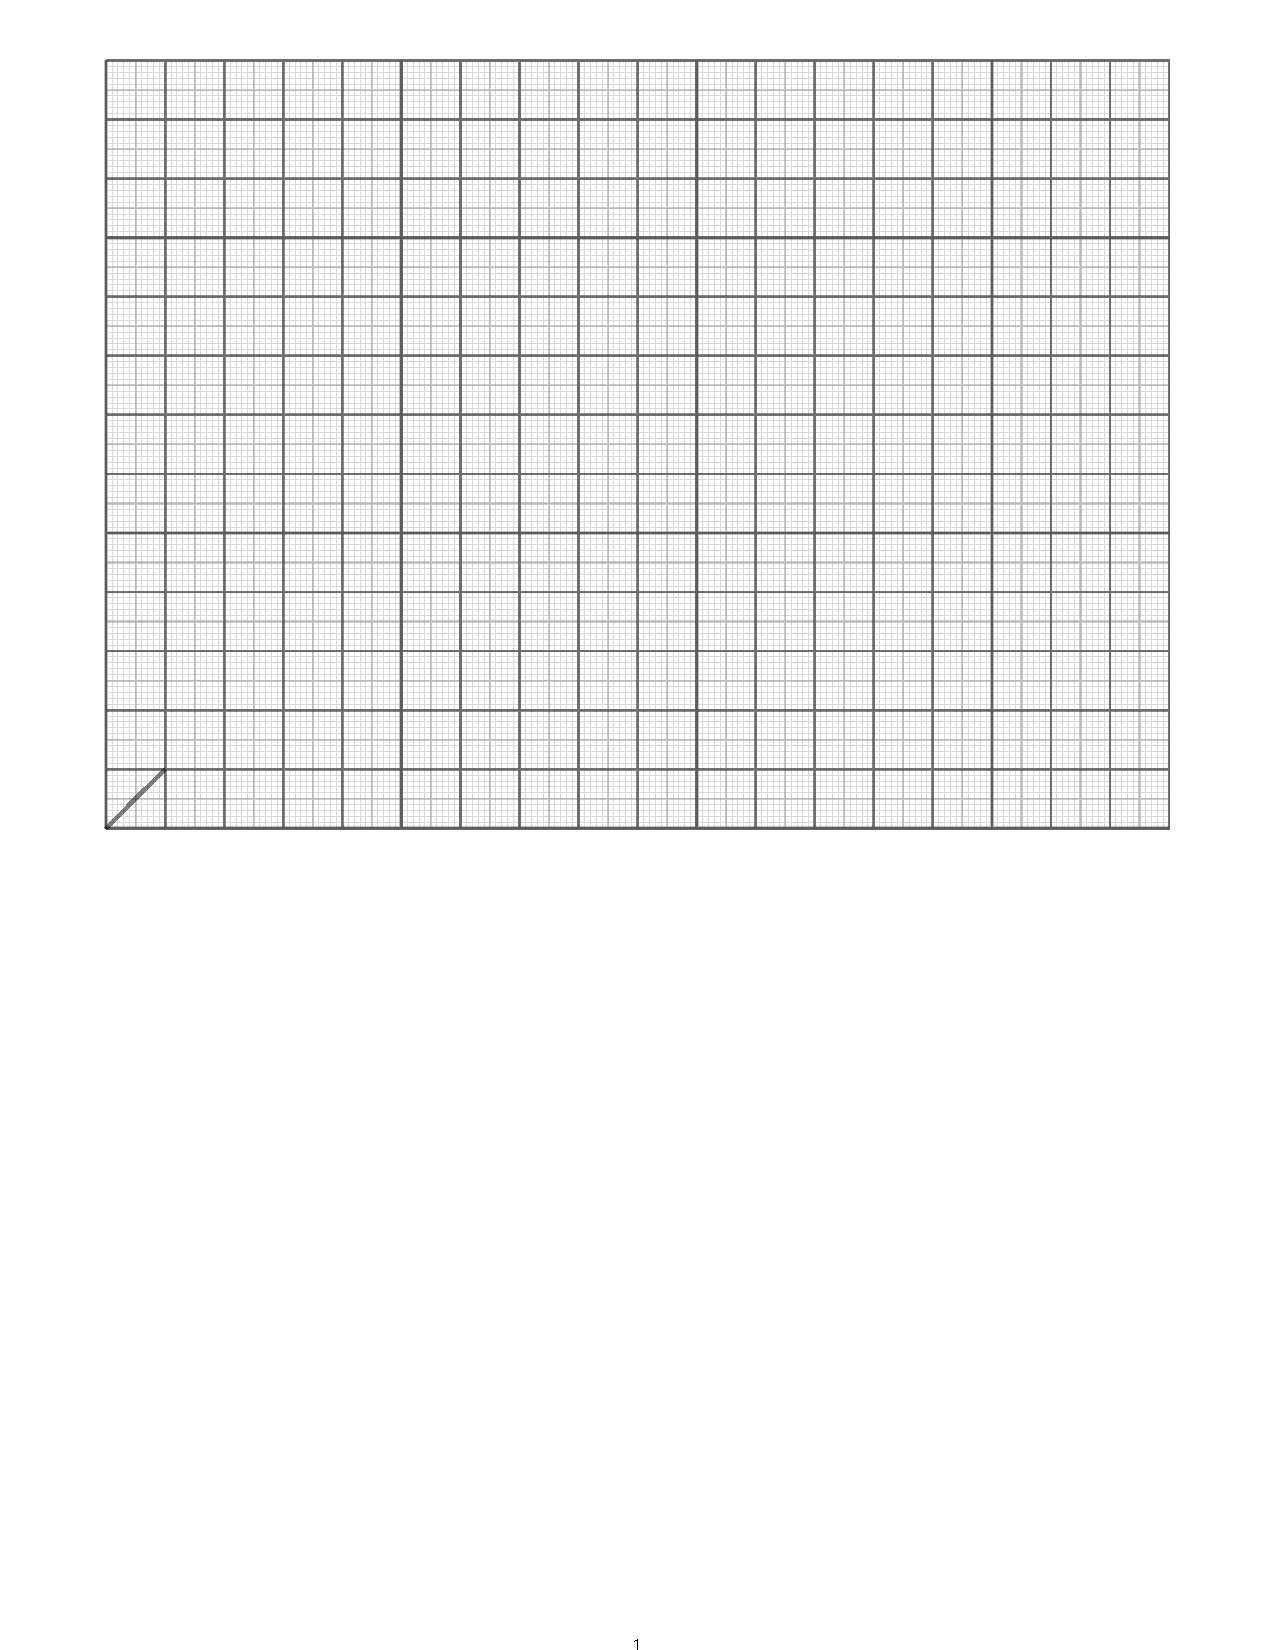
\includegraphics[width=0.7\linewidth]{ex5}};
		
		\draw[step=1mm, line width=0.1mm, black!30!white] (0,0) grid (\width,\hauteur);
		\draw[step=5mm, line width=0.2mm, black!40!white] (0,0) grid (\width,\hauteur);
		\draw[step=5cm, line width=0.5mm, black!50!white] (0,0) grid (\width,\hauteur);
		\draw[step=1cm, line width=0.3mm, black!90!white] (0,0) grid (\width,\hauteur);
		
		\draw[ultra thick] (0,0) -- (1,1) ;
		
		
		\end{tikzpicture}
	\end{center}
\end{document}